\section{System}\label{design}

\subsection{Data Cleanup}

The data source I have used for my project is the wines database belonging to Decanter.com\cite{DecanterCom}. The database contains nearly 40,000 professional ratings and tasting notes for wines from as far back as 1986, featuring vintages as far back as 1917.

The original database is highly inconsistent, displaying a mixture of design approaches and a variable quality of data. This is consistent with the fact that the database has been developed over a long period of time by a number of different developers with varying levels of skill, and that wine journalists making entries into the database have taken a number of idiosyncratic approaches to data entry.

Nevertheless I considered there to be a great deal of useful and interesting information in the database, with it to contain usable ratings and/or tastings for over 33,000 wines.

\subsection{The Decanter Database}

\begin{figure}[h!]
    \caption{Decanter.com Database}
    \centering
        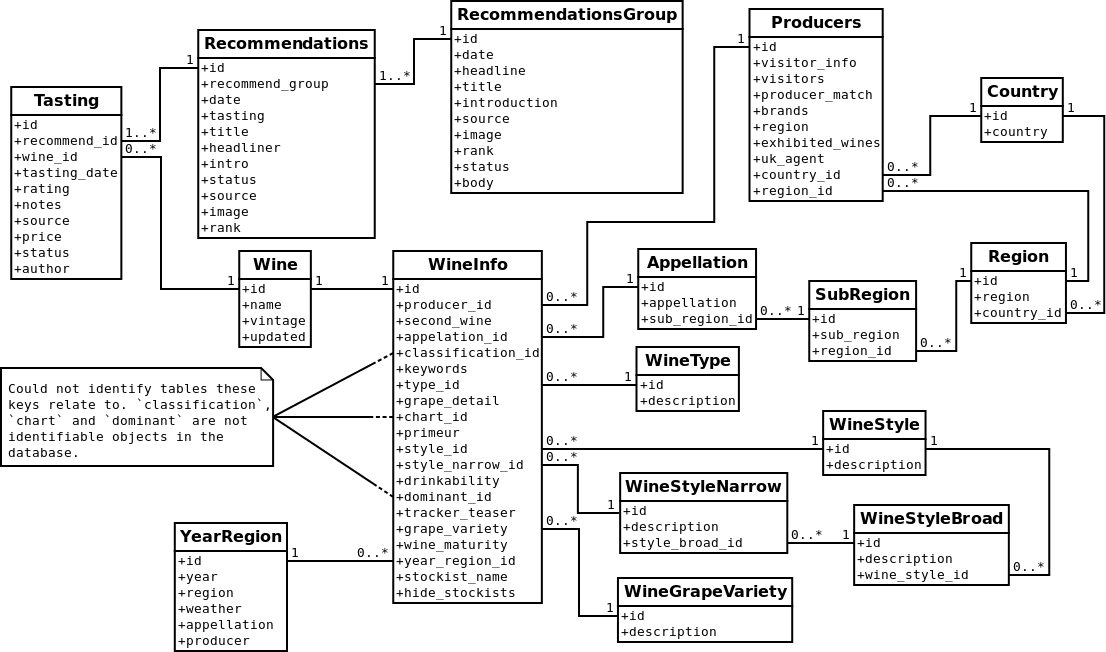
\includegraphics[width=14cm]{DecanterWineDB}
    \label{fig:decanterdb}
\end{figure}

In the original database the WineInfo table is a mixture of foreign keys joining to very small tables, such as WineInfo.type\_id joining to WineType.id where WineType is a table with only two attributes. This approach, stiving for a high degree of normalisation, contrasts with the fact that the same table also has the attribute second\_wine, as a string which only holds data in 450 of the 38762 entries in the table.

\subsection{Creating The Sommelier Dataset}

\begin{figure}[h!]
    \caption{Sommelier Database}
    \centering
        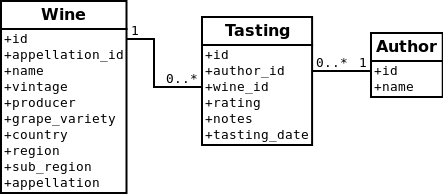
\includegraphics[width=7cm]{SommelierDBSimple}
    \label{fig:sommelierdb}
\end{figure}

For the new Sommelier database, Figure \ref{fig:sommelierdb}, I decided to denormalise [explanation/citation needed!] the wine data. This enables the data to be queried with fewer joins, maximising the simplicity and execution speed of the queries [citation needed] used for data access. Denormalization makes data integrity more difficult to maintain however, as there are potentially a large number of records to update for any change in a duplicated value. In this case an appellation or sub-region name changing might require thousands of records to be amended. Creating and editing wines is not a requirement of my system though, so for the purposes of this project the wine and tasting data is static and will not be subject to updates. For this reason the duplication of data within the Wine records is not problematic. In a real world setting this issue may need to be revisited.

Much of the data from the original database was disregarded entirely.

The tables WineStyleNarrow and WineStyleBroad contained generic text descriptions for wine (``rich and creamy'', ``crisp and tangy'' etc.). I initially considered this to have potential for migration into tag data which I could reuse as part of my filtering. Unfortunately less than 6435 of the records in WineInfo had non-null values for their style\_narrow\_id field, and only 3397 of these had corresponding records in the Tasting table. This figure was only around 10\% of the number of wines I expected the Sommelier database to contain so I decided that the WineStyle* tables were probably not worthwhile to migrate.

The WineType table was ignored because no wines corresponded to it; no WineInfo.type\_id record matched any WineType.id.

The TasterRating and TastingId tables were discarded because they only referenced 1158 of the records in Tasting, too small a proportion of the Tasting table to make it worthwhile migrating them into the dataset.

\subsection{The Author Problem}

The biggest shortcoming of the dataset is that the author of a tasting note is often not recorded. The number of wines with notes and known authors is only 1401, with there being 18 named authors on the system. 

Table \ref{table:authors} shows the distribution of tastings amongst authors, only 5 of which have tasted and rated more than 100 wines in the database.

\begin{table}[ht]
    \caption{Authors of tasting notes and ratings}
    \centering
    \begin{tabular}{c c c}
        \\\hline\hline
        Author               & Wines tasted & Wines also tasted by another
        \\\hline
        Amy Wislocki         &           28 & 1  \\
        Andrew Jefford       &          105 & 38 \\
        Beverley Blanning MW &           13 & -  \\
        Carolyn Holmes       &            1 & -  \\
        Christelle Guibert   &          119 & 9  \\
        Clive Coates MW      &            6 & -  \\
        David Peppercorn     &           44 & -  \\
        Gerald D Boyd        &            7 & -  \\
        Harriet Waugh        &          250 & 23 \\
        James Lawther MW     &          226 & 21 \\
        John Radford         &            2 & -  \\
        Josephine Butchart   &           24 & 1  \\
        Norm Roby            &            4 & -  \\
        Rosemary George MW   &            6 & -  \\
        Serena Sutcliffe     &           31 & 15 \\
        Stephen Brook        &           19 & 3  \\
        Steven Spurrier      &          497 & 53 \\
        \\\hline
    \end{tabular}
    \label{table:authors}
\end{table}

\begin{table}[ht]
    \caption{Matrix of authors with wines tasted in common}
    \centering
    \begin{tabular}{c c c c c c c c c c}
        \\\hline\hline
        Author                   & SS & JL & JB & SB & CG & SS & HW & AJ & AW
        \\\hline
        Steven Spurrier (SS)     & -  & 6  & 1  & 1  & 7  & 0  & 15 & 30 & 1 \\
        James Lawther MW (JL)    & 6  & -  & 0  & 0  & 0  & 15 & 0  & 0  & 0 \\
        Josephine Butchart (JB)  & 1  & 0  & -  & 0  & 0  & 0  & 0  & 0  & 0 \\
        Stephen Brook (SB)       & 1  & 0  & 0  & -  & 0  & 0  & 1  & 1  & 0 \\
        Christelle Guibert (CG)  & 7  & 0  & 0  & 0  & -  & 0  & 1  & 5  & 0 \\
        Serena Sutcliffe (SS)    & 0  & 15 & 0  & 0  & 0  & -  & 0  & 0  & 0 \\
        Harriet Waugh (HW)       & 15 & 0  & 0  & 1  & 1  & 0  & -  & 10 & 0 \\
        Andrew Jefford (AJ)      & 30 & 0  & 0  & 1  & 5  & 0  & 10 & -  & 0 \\
        Amy Wislocki (AW)        & 1  & 0  & 0  & 0  & 0  & 0  & 0  & 0  & - \\
        \\\hline
    \end{tabular}
    \label{table:authormatrix}
\end{table}

In some cases an author's initials or full name are recorded within the text of a tasting note. I decided that extracting and making use of these was impractical given the time constraints of this project.

DESCRIBE DATA SETS BEFORE AND AFTER

THE SOMMELIER DATASET

Having analysed the dataset and conceived an ideal schema, I needed to decide what the criteria to apply when extracting my new dataset from the source data.

Given that the purpose of the dataset is social recommendations, the first decision I made was to discard any wines without both tasting notes and a rating, whether.

\subsection{Making Recommendations}

Wine attributes, vintage, grape variety, region etc., are of limited use for making recommendations. Take a user who has rated a red Bordeaux wine highly. It is not interesting to that user for a system to simply recommend them other highly-rated red Bordeaux wines, which is what a system will do if it looks for items with similar attributes. It is likely that any drinker who enjoys Bordeaux wines will recognise that such wines are of a type, with geography, grape varieties and production processes in common. Thus the user will be capable of ``recommending'' Bordeaux wines to themselves, and will not have very much difficulty sourcing ones which are highly rated. They do not need a recommender system for that.

It is recommendations in spite of the attributes of the subject item that are of real interest. Recommending a Syrah from Chile's Colchagua Valley to someone who rated a red Bordeaux wine highly might be of more interest. It is relatively more likely that a user is unaware of the fine Syrah wines from that region, and that makes it a much more interesting recommendation; potentially a good one.

Similarly a recommendation of another Bordeaux red wine might be good, as long as it were possible to establish a commonality of appeal for that particular drinker other than that the wine is similar in attributes. For example there are many delicious Pauillacs from 2005, made of the same grape varieties in the same manner; finding the one which is most interesting to a given user is not aided by looking at its grape variety or appellation as they are identical. The appeal and interest of a wine recommendation lies in qualities beyond the item's attribute profile.

So, by disregarding the attributes of the wines it may be possible to make more interesting recommendations.

A corrollary benefit of this disregard for wine attributes is that I am able to make use of far more of the Decanter.com data, many of the wines within which have incomplete attributes.

TODO appendix of data


1. select a.name, count( t.id ) from author a join tasting t on a.id = t.author\_id where 0 < ( select count(*) from tasting t2 where t2.winei\_id = t
.wine\_id and t2.author\_id <> 0 and t2.author\_id <> t.author\_id)  group by a.id;                                                                        
+--------------------+---------------+
| name               | count( t.id ) |
+--------------------+---------------+
| Steven Spurrier    |            53 |
| James Lawther MW   |            21 |
| Josephine Butchart |             1 |
| Stephen Brook      |             3 |
| Christelle Guibert |             9 |
| Serena Sutcliffe   |            15 |
| Harriet Waugh      |            23 |
| Andrew Jefford     |            38 |
+--------------------+---------------+

2. select a.name, count( t.id ) from author a join tasting t on a.id = t.author\_id where 0 < ( select count(*) from tasting t2 where t2.wine\_id = t.wine\_id and t2.author\_id = {N} ) group by a.id; 

\subsection{Experimentation}

In Chapter 2 of Collective Intelligence\cite{Segaran02}, Segaran details basic methods for user- and item-based collaborative filtering. Following the guidelines from this chapter I recreated Segaran's recommendation methods and applied them to my dataset.

\begin{table}[ht]
    \caption{Pearson Similarity of Authors}
    \centering
    \begin{tabular}{c c c c c c c c c c}
        \\\hline\hline
        Author                   & SS   & JL   & JB  & SB  & CG  & SS  & HW   & AJ   & AW
        \\\hline
        Steven Spurrier (SS)     & -    & 0.58 & 0.0 & 0.0 & 0.0 & -    & 0.67 & 0.49 & 0.0 \\
        James Lawther MW (JL)    & 0.58 & -    & -   & -   & -   & 0.22 & -    & -    & -   \\
        Josephine Butchart (JB)  & 0.0  & -    & -   & -   & -   & -    & -    & -    & -   \\
        Stephen Brook (SB)       & 0.0  & -    & -   & -   & -   & -    & 0.0  & 0.0  & -   \\
        Christelle Guibert (CG)  & 0.0  & -    & -   & -   & -   & -    & 0.0  & 0.0  & -   \\
        Serena Sutcliffe (SS)    & -    & 0.22 & -   & -   & -   & -    & -    & -    & -   \\
        Harriet Waugh (HW)       & 0.67 & -    & -   & 0.0 & 0.0 & -    & -    & 0.71 & -   \\
        Andrew Jefford (AJ)      & 0.49 & -    & -   & 0.0 & 0.0 & -    & 0.71 & -    & -   \\
        Amy Wislocki (AW)        & 0.0  & -    & -   & -   & -   & -    & -    & -    & -   \\
        \\\hline
    \end{tabular}
    \label{table:authormatrix}
\end{table}

N.B.

Table data obtained by:

from lib import recommendations
authorsims = recommendations.getAuthorSimilarities()


\subsection{Implementation}

\begin{figure}[h!]
    \caption{Sommelier Class Diagram}
    \centering
        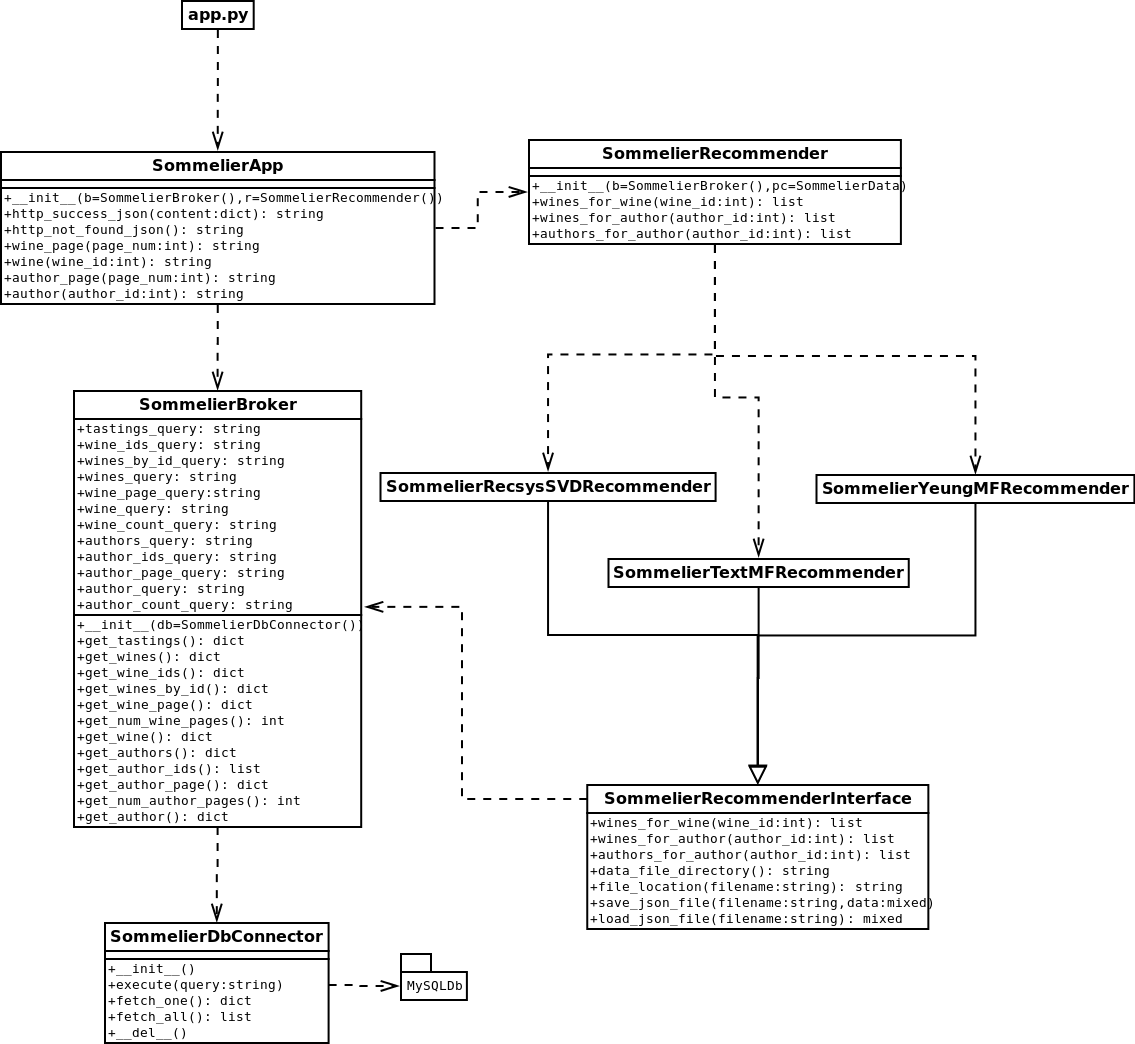
\includegraphics[width=15cm]{SommelierClassDiagram}
    \label{fig:sommelierclasses}
\end{figure}

Having so few wines tasted by more than one author in the dataset, and even fewer tasted by more than two, it was clear that my system needed to cope extremely well with sparsity. Su et al. \cite{SuImputed} show their \ldots

!!! Would have been quixotic to attempt a complex approach involving text mining of tasting notes without first attempting to approximate the state of the art in imputation of preferences using matrix factorization, or a Bayesian approach\ldots

!!! I decided firstly to imitate Su et al.'s \cite{SuImputed} IDN-CF (eBMI) method (imputed densest neighbours collaborative filtering using extended Bayesian multiple imputation). This approach has been shown to mitigate the problem of sparsity, requiring very few neighbours to obtain its best recommendations compared to other methods. 

!!! The IDN-CF (eBMI) implementation only utilizes the rating component of a tasting note, whereas I had set myself the objective of finding a use for the tasting note itself. Initially it occurred to me that I could build a Bayesian classifier, or similar, to identify \ldots Hu and Zhou (2008) etc.




